\documentclass{article}

% Language setting
% Replace `english' with e.g. `spanish' to change the document language
\usepackage[english]{babel}


% Set page size and margins
% Replace `letterpaper' with `a4paper' for UK/EU standard size
\usepackage[a4paper,margin=2.5cm]{geometry}

% Header and footer Package
\usepackage{fancyhdr}

% Useful packages
\usepackage{amsmath}
\usepackage{graphicx}
\usepackage[colorlinks=true, allcolors=blue]{hyperref}
\usepackage{caption}
\usepackage{subcaption}
\usepackage{float}
\usepackage{listings}
\usepackage{algorithm,algorithmicx,algpseudocode}

\newcommand{\course}{Symmetric Cryptography}
\newcommand{\me}{João Gaspar (025605833A)}
\newcommand{\labName}{Homework 4: Hash Functions and MAC}
\date{}

\fancyhead[L]{\course - \labName}
\fancyhead[R]{\me}
\pagestyle{fancy}
\title{\textit{\course} - \labName}
\author{\me}


\begin{document}
\maketitle
\section{Cascading Hash Functions}
\subsection{Describe an algorithm capable of finding collisions in H in time significantly less than $2^{n}$}
Let $f$ be the compressing algorithm of $H$, and $d$ the block\_size.\\
We know also that $H(x) = f^{(t)}(h_{t-1} || x)$, where $t$ is the number of iterations of $f$ that is equal to $\frac{\text{len}(x)}{d} + 1$ as we append the size to the messagee.
\begin{enumerate}
    \item Choose a random $b$ of size $d$
    \item Compute $h_1 = f(h_0 || b)$.
    \item Check if $h_1$ is in the table.
    \item If it is and $b \neq b'$, then:
        \begin{enumerate}
            \item We have found a collision for $f^{(i)}$.
            \item Stop procedure
        \end{enumerate}
    \item Else, we add $h_1$ to the table with the corresponding block $b$ and repeat the process.
\end{enumerate}

This operation takes $O(2^{n/2})$ time per block and has space complexity of $O(2^{n/2})$ according to birthday paradox to have around $50\%$ of chance of finding a match.
And we can repeat this process for $t=n/2$ iterations, using the output of the previous iteration as the input for the next one such that we will have $O(\frac{n}{2} \cdot 2^{(n/2)})$ time complexity that yields $2^{t} = 2^{(n/2)}$ collisions for $H_1$, as we obtain $t$ blocks pairs that collide for $f$ and we can combine them to obtain $2^{t}$ collisions for $H_1$. Moreover, since Merkle-Damgard construction is recursive process, and since our collision blocks have the same size, we can finalize the process by concatenating the length of the blocks to the end of the message, and we will still have these collisions for $H_1$.

Now, for $H_2$, we know that if we apply a birthday attack, we will probably find a collision in $O(2^{n/2})$ time. Since that we in the first proccess acquired $2^{(n/2)}$ collisions for $H_1$, we can use those collisions to find a collision for $H_2$ in $O(2^{n/2})$ time, as per the birthday paradox we have a good chance that we will find a collision with this number of test elements.

This makes the attack on $H$ to be $O(\frac{n}{2} 2^{n/2}) + O(2^{n/2})$ that is equal to $O(\frac{n+1}{2} 2^{n/2}) = O(n \cdot 2^{n/2})$ time complexity, which is significantly faster than $O(2^{n})$. Note also that the space complexity of this attack is just $O(2n) = O(n)$, as we just need to store the pair of blocks that collide for $H_1$, ie. $b_i$ and $b_i'$, as we just have to permute them to find all the candidates for the collision of $H_1$.

\subsection{How efficiently can you find collisions for H(x) with an extra hash functions?}
We can repeat the exact same process as before, but with more collisions for the Merkle-Damgard, as we now need to find collisions for $H_2$ and $H_3$ at the same time.
as we've seen before, we needed $2^{n/2}$ candidates to find a collision for an hash function with codomain of size $n$ with a good probability, and since we now have 2 hash functions to find a collision for, we have a codomain of size $2n$, therefore we will need $2^{(2n)/2} = 2^{n}$ candidates to find a collision for both $H_2$ and $H_3$ with a good probability. This leads to a time complexity of $O(n \cdot 2^{n/2})\text{ to gather the colision candidates } + O(2^{n})$ to test all candidates for a collision. This is still better than brute-force attack relying on the birthday paradox as it would take $O(2^{(3n)/2})$ time.

\section{Collisions for Hash Functions}
To find a collision for the given hash function, we can use a birthday attack, which naïvely required saving the random hashes leading to a time complexity of $O(2^{48/2})$ and memory complexity of $O(2^{48/2})$. But, as shown in class if cojoined with a cycle detection algorithm, we can find a collision in $O(2^{48/2})$ time and $O(1)$ memory.

The idea is to start with two pointers, one that steps once per iteration (tortoise) and another that steps twice per iteration (hare).
We start both pointers at the same random message \\
($=JOAO||random\_string$), and then we move the tortoise one step at a time and the hare two steps at a time, until they meet. Once they meet, we know that there is a cycle in the sequence of hashes.

\begin{lstlisting}[language=Python]
def step(digest: bytes) -> bytes:
    return hash_message(NAME + digest)

initial = fast = slow = step(random.randbytes(8))
fast = step(step(fast))
slow = step(slow)

# Note: In my code I used a for loop to use tqdm
#       to show the progress of the attack
while fast != slow:
    fast = step(step(fast))
    slow = step(slow)
\end{lstlisting}

(Note: the following proof was made in my own interest and was not part of discovering the solution, as the solution was shown in class, and I wanted to understand why it worked.)

Now we know that the slow pointer has taken $k$ steps and the fast pointer has taken $2\cdot k$ steps.\\
Let $l_{nc}}$ be the length of the non-cyclic part of the sequence and $l_{c}$ the length of the cycle.\\
We know from some integers $i,j$:
\begin{equation}
    \begin{aligned}
    \begin{cases}
        k &= l_{nc} + i \cdot l_{c} \\
        2k &= l_{nc} + j \cdot l_{c}
    \end{cases} \Leftrightarrow
    k &= 0 + (j-i) \cdot l_{c} \Leftrightarrow
    k \equiv 0 \mod l_c

    \end{aligned}
\end{equation}
So k is a multiple of $l_{c}$

We also know that the meeting point must be at a distance of $d = k - l_{nc} \mod l_c$ from the beginning of the cycle.\\
Simplifying, we have $d = -l_{nc} \mod l_c$.\\
Therefore, if we walk $l_{nc}$ steps from the initial point, we know that we will be in the beginning of the cycle, furthermore, if we walk $l_{nc}$ steps from the meeting point, then we will also be in the beginning of the cycle, as:
\begin{equation}
    d + l_{nc} \equiv -l_{nc} + l_{nc} \mod l_c \equiv 0 \mod l_c
\end{equation}


\begin{lstlisting}[language=Python]
finder = initial
for _ in tqdm(
    infinite_loop(),
    desc="Finding Collision",
    unit="attempts",
    total=2**24,  # birthday bound is 2**24
):
    nf = step(finder)
    ns = step(slow)
    if nf == ns and slow != finder:
        break  # Collision found
    finder = nf
    slow = ns

print("Collision found!")
print(f"Message 1: {NAME.decode()}||{finder.hex()}")
print(f"Message 2: {NAME.decode()}||{slow.hex()}")
print(f"Hash 1: {hash_message(m1).hex()}")
print(f"Hash 2: {hash_message(m2).hex()}")
\end{lstlisting}


\begin{lstlisting}[language=Python]
Finding Cicle: 93% | {progress bar} | 15520189/16777216
Finding Collision: 52%| {progress bar} | 8785338/16777216
Collision found!
Message 1: Joao||5e5b39d274b7
Message 2: Joao||92c489a4bdd7
Hash 1: 5b272d64b94f
Hash 2: 5b272d64b94f
\end{lstlisting}

\section{Meaningful Second Preimage}
I've written the following text:\\
\begin{center}
    \textit{``Hash functions are functions that take an arbitrarily sized input and produce a fixed size output. They are an essential component of modern cryptography.''}
\end{center}

My first idea was to flip random bits in the message, but this would disrupt the meaning of the message and potentially make it unreadable, and then I thought about synonyms, which would indeed keep the meaning of the text, so I would have to choose for example 8 words in the text that have each 4 synonyms, and then I would have $4^8 = 2^{16}$ candidates for the second preimage, which is enough to find a collision, I ended up choosing a substitute for almost every word giving me $2^8 \cdot 3^{10} = 15'116'544 \approx 2^{23.85}$ alternatives, such that the probability of a 16-bit value having no pre-image was almost negligible (there are $2^{16}$ images).
We successfully can find significant second preimages for the given hash function, as we can see in the following output, where we have a message with the same hash value as provided by the user, where the message is diffeerent but still has the same meaning as the original message and is readable:

\begin{lstlisting}[language=bash]
$ python3 Ex3.py 8008
Message hash: 374b
Target  hash: 8008
159638it [00:00, 222475.14it/s]                                                                                        
Found a collision:
Hash functions are functions that take a varying length input and produce a
single constant size digest. Such functions represent a key element of
modern cryptography.
With hash: 8008
\end{lstlisting}

Now we have to make sure that our program has the same hash value as \texttt{SHA256("Joao")}. To achieve this, I've created a script called \texttt{Ex3\_filehash.py}. This script reads the content of \texttt{Ex3.py} and then it keeps calculating the hash of the file plus a newline with a comment containing the hex representation of random bytes until it finds a hash value that is equal to \texttt{SHA256("Joao")}.\\

When verifying the hash of the file, we can see that it is indeed equal to \texttt{SHA256("Joao")}, and therefore we have successfully found a second preimage for the given hash function, where the message is the content of \texttt{Ex3.py} and the hash value is the same as \texttt{SHA256("Joao")}:

\begin{lstlisting}[language=bash]
$ echo -n "Joao" | sha256sum
5f2e5aa5c388a6df41ff3c32531d4d81a661487bacadc010a4b6cdca0a7eb04d  -
$ sha256sum Ex3.py
5f2e77f42f74d5d5f65e0f5e6729f3c0b53cb7dd26bba082770bab2ba0dc60eb  Ex3.py
\end{lstlisting}


\section{Second Preimage Resistance of Sponge}
Initially we are given the message $m$, and the sponge internal state consisting of the size of $r$, $c$ and the permutation $f$.
We want to find a message $m' \neq m$ such that $sponge(m) = sponge(m')$ in an algorithm that has time complexity of $O(2^{c/2})$ in terms of calls to $f$ or $f^{-1}$.\\
Moreover, $f$ is invertible.

To achieve this, we know that we have to build a birthday attack on an image of $C$ bits, to give us the time complexity of $O(2^{c/2})$.
The idea to find a collision on the capacity part of the state and not the whole state is that we have direct access to the rate part of the state allowing us to control its value so that it matches the pre-image of the $f$ function.

We can start by calculating every intermediate state of the sponge function for the message $m$, and we can store these states in a table with the corresponding index of the block that we are processing.
This gives us a table of $c_i \rightarrow (r || c_{i-1}, i)$, ie. passing the state $r || c_{i-1}$ through the function $f$, we will obtain $S_i = r_i || c_i$. This index $i$ is needed to trace back the path of the message $m$ through the sponge function.
This will however not be enough, as we need a good chance of having a collision, by finding $O(2^{c/2})$ candidates.
To find more candidates, we can, for all $S_i$ in the table, obtain $S_j = f^{-1}(S_i \oplus (r || 0^c))$ and store the resultant capacity in the table, and repeat this process to the newly obtained list of $S_j$'s until we have $O(2^{c/2})$ candidates for the collision, which is enough to find a collision with good probability.

This allows us to have $O(2^{c/2})$ candidates for the collision, as we have $O(2^{c/2})$ states in the table, taking $O(2^{c/2})$ time and $O(2^{c/2})$ space complexity to build.

Now, we can start testing random candidates for the collision, by generating random $r'$ and calculating $S' = f(r' || 0^c)$, and checking if $c'$ is in the table.\\
If it is, we have found a collision for the capacity part of the state (we will call $S_i$ to the element on the table that collided with $S'$).\\
This means that we have found $S'$ such that $\text{capacity of }f(S') =\text{ capacity of } S_i$ 

We can build our second preimage $m'$ by: 
\begin{enumerate}
    \item Set the first block of $m'$ to be $r'$
    \item Get rate bits of $f(S') = x$ and rate bits of $S_i = r_i$
    \item Set the second block of $m'$ to be $x \oplus r_i$
    \item Set the remaining blocks of $m'$ to be equal to the remaining $m_i$ of the path of $S_i$.
\end{enumerate}
We will obtain: $r' || (x \oplus r_i) || m_i || ... || m_{\lfloor \frac{m}{r} \rfloor + 1}$ which will hash to the same value.

\section{PMAC Variant}
First let $E_k_1(m_i \oplus E_k_2(i)) = E_i(m)$ representing encryption of block $m$ at position $i$.\\
Per the construction, and simplifying by ignoring CRC-128 function, we will have, for a message $m$ with 4 blocks:
$\text{\textit{MAC}}(m) = E_0(m_1) \oplus E_1(m_2) \oplus E_2(m_3) \oplus E_3(m_4) \oplus E_4(\text{padding})$

Therefore, if we get $E_0(m_1)$, $E_1(m_2)$, $E_2(m_3)$, $E_3(m_4)$ and $E_4(\text{padding})$, by utilising the signing oracle, we can combine them to oobtain the MAC of the message $m$.

I want to sign: ``Hello, I am $<$Joao$>$ and this is my cryptohomework'', which was especially created to have 4 blocks of 16 bytes, as we use AES-128, so that we both dont have to worry about different paddings (they will be always 16 bytes of $0x10$) and so that no blocks have both angular brackets.

Before querying the signing oracle, let $A$ be the message containing 16 A's.

Now, querying the signing oracle for the following messages we will obtain the following MACs:
\begin{enumerate}
    \item $m_1$: ``Hello, I am $<$Joa''
        \begin{enumerate}
            \item MAC: $380b598be0366e85083dc581d2a210ce$
            \item Result: $E_0(m_1) \oplus E_1(\text{padding})$
        \end{enumerate}
    \item $m_2$: ``$A||$o$>$ and this is m''
        \begin{enumerate}
            \item MAC: $673d03a683c72ccc066f1f1ccb904e79$
            \item Result: $E_0(A) \oplus E_1(m_2) \oplus E_2(\text{padding})$
        \end{enumerate}
    \item $m_3$: ``$A||A||$y cryptohomework''
        \begin{enumerate}
            \item MAC: $33d32bfb932cea176dc24b4d9ef4f075$
            \item Result: $E_0(A) \oplus E_1(A) \oplus E_2(m_3) \oplus E_3(\text{padding})$
        \end{enumerate}
\end{enumerate}
Now, we can combine these MACs to obtain the MAC of the message $m$:
\begin{equation}
    \begin{aligned}
        \text{\textit{MAC}}(m) = &E_0(m_1) \oplus E_1(\text{padding}) \\
            \oplus &E_0(A)    \oplus E_1(m_2)            \oplus E_2(\text{padding}) \\
            \oplus &E_0(A)   \oplus E_1(A)              \oplus E_2(m_3)           \oplus E_3(\text{padding}) \\
    \end{aligned}
\end{equation}
We can sucessfully remove $E_0(A)$, but we are left with $E_1(\text{padding})$, $E_2(\text{padding})$ and $E_1(A)$ that shouldn't be on the final message.
To remove them, I created two more messages to be signed by the signing oracle:
\begin{enumerate}
    \item{ ``$A$''
        \begin{enumerate}
            \item MAC: $0bb89ccaa4b6c48fb920b04d53fcf64c$
            \item Result: $E_0(A) \oplus E_1(\text{padding})$
        \end{enumerate}
    }
    \item{ ``$A||A$''
        \begin{enumerate}
            \item MAC: $2066f871bb8d2432411ff16ba454854d$
            \item Result: $E_0(A) \oplus E_1(A) \oplus E_2(\text{padding})$
        \end{enumerate}
    }
\end{enumerate}

Now by combining these new MACs with the previous ones, we can remove the unwanted terms and obtain the MAC of the message $m$:
\begin{equation}
    \begin{aligned}
        \text{\textit{MAC}}(m) = &E_0(m_1) \oplus E_1(\text{padding}) \\
            \oplus &E_0(A)\ \  \oplus E_1(\text{padding}) \\
            \oplus &E_0(A)\ \  \oplus E_1(m_2)        \oplus E_2(\text{padding}) \\
            \oplus &E_0(A)\ \  \oplus E_1(A) \ \            \oplus E_2(m_3)           \oplus E_3(\text{padding}) \\
            \oplus &E_0(A)\ \ \oplus E_1(A)\ \ \oplus E_2(\text{padding}) \\
            =& E_0(m_1) \oplus E_1(m_2)\ \oplus E_2(m_3) \oplus E_3(\text{padding}) \\
            =& \text{\textit{MAC}}(m)
    \end{aligned}
\end{equation}

But this is a simplified solution as said before, therefore we have to revert the CRC-128 function in all obtained MACs and then combine them so to obtain the MAC of the forged message.

To do so, we were given an hint that CRC-128 is an affine function, ie. $\text{CRC-128}(m) = A \cdot m \oplus b$, therefore
\begin{equation}
\begin{aligned}
                \text{MAC}(M) = A \cdot E(M) + b \\
                \Rightarrow \text{MAC}(M_1) \oplus \text{MAC}(M_2) &= A \cdotE(M_1) \oplus b \oplus A \cdot E(M_2) \oplus b  \\
                                                                   &= A \cdot E(M_1) \oplus A \cdot E(M_2)\\
                                                                   &= A \cdot (E(M_1) \oplus E(M_2))

\end{aligned}
\end{equation}
Which is invalid since the $b$ term disappeared, however if we have an odd number of messages, for instance 3, the $b$ term will be present such that it's now a valid signature for the message $M_1 \oplus M_2 \oplus M_3$.

And since I have 5 messages: ($m_1$, $m_2$, $m_3$, $A$ and $A||A$), I can combine them to obtain the MAC of the message $m$ by simply XORing all the obtained MACs.

\begin{equation}
\begin{aligned}
    &\text{\textit{MAC}}(\text{``Hello, I am <Joao> and this is my cryptohomework''}) \\
    =&\text{MAC}(m_1) \oplus \text{MAC}(m_2) \oplus \text{MAC}(m_3) \oplus \text{MAC}(A) \oplus \text{MAC}(A||A) \\
    =&380b598be0366e85083dc581d2a210ce \\
    \oplus &673d03a683c72ccc066f1f1ccb904e79 \\
    \oplus &33d32bfb932cea176dc24b4d9ef4f075 \\
    \oplus &0bb89ccaa4b6c48fb920b04d53fcf64c \\
    \oplus &2066f871bb8d2432411ff16ba454854d \\
    =&473b156defe648e39bafd0f6706eddc3
\end{aligned}
\end{equation}

And effectively, when we verify the signature of the message with the signature:

$473b156defe648e39bafd0f6706eddc3$

We see that the signature is valid, and therefore we have successfully forged a signature for the message.

\begin{flushleft}
\begin{aligned}
\text{hex}(\text{message}) =\ &48656c6c6f2c2049 \\
                              &20616d203c4a6f61 \\
                              &6f3e20616e642074 \\
                              &686973206973206d \\
                              &792063727970746f \\
                              &686f6d65776f726b &&
\end{aligned}
\end{flushleft}


\begin{figure}[h]
    \centering
    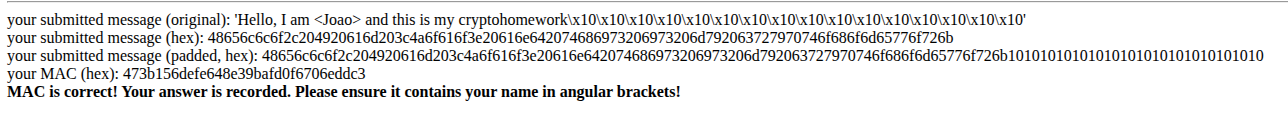
\includegraphics[width=\textwidth]{figures/MAC}
    \caption{Forged signature.}
\end{figure}



\end{document}
